%%%%%%%%%%%%%%%%%%%%%%%%%%%%%%%%%%%%%%%%%%%%%%%%%%%%%%%%%%%%%%%%%%%%%%
% LaTeX Example: Project Report
%
% Source: http://www.howtotex.com
%
% Feel free to distribute this example, but please keep the referral
% to howtotex.com
% Date: March 2011 
% 
%%%%%%%%%%%%%%%%%%%%%%%%%%%%%%%%%%%%%%%%%%%%%%%%%%%%%%%%%%%%%%%%%%%%%%
% How to use writeLaTeX: 
%
% You edit the source code here on the left, and the preview on the
% right shows you the result within a few seconds.
%
% Bookmark this page and share the URL with your co-authors. They can
% edit at the same time!
%
% You can upload figures, bibliographies, custom classes and
% styles using the files menu.
%
% If you're new to LaTeX, the wikibook is a great place to start:
% http://en.wikibooks.org/wiki/LaTeX
%
%%%%%%%%%%%%%%%%%%%%%%%%%%%%%%%%%%%%%%%%%%%%%%%%%%%%%%%%%%%%%%%%%%%%%%
% Edit the title below to update the display in My Documents
%\title{Project Report}
%
%%% Preamble
\documentclass[paper=a4, fontsize=11pt]{scrartcl}
\usepackage[T1]{fontenc}
\usepackage{fourier}

\usepackage[english]{babel}															% English language/hyphenation
\usepackage[protrusion=true,expansion=true]{microtype}	
\usepackage{amsmath,amsfonts,amsthm} % Math packages
\usepackage[pdftex]{graphicx}	
\usepackage{url}
\usepackage{graphicx}
\usepackage{float}

%%% Custom sectioning
\usepackage{sectsty}
\allsectionsfont{\centering \normalfont\scshape}


%%% Custom headers/footers (fancyhdr package)
\usepackage{fancyhdr}
\pagestyle{fancyplain}
\fancyhead{}											% No page header
\fancyfoot[L]{}											% Empty 
\fancyfoot[C]{}											% Empty
\fancyfoot[R]{\thepage}									% Pagenumbering
\renewcommand{\headrulewidth}{0pt}			% Remove header underlines
\renewcommand{\footrulewidth}{0pt}				% Remove footer underlines
\setlength{\headheight}{13.6pt}


%%% Equation and float numbering
\numberwithin{equation}{section}		% Equationnumbering: section.eq#
\numberwithin{figure}{section}			% Figurenumbering: section.fig#
\numberwithin{table}{section}				% Tablenumbering: section.tab#


%%% Maketitle metadata
\newcommand{\horrule}[1]{\rule{\linewidth}{#1}} 	% Horizontal rule

\title{
		%\vspace{-1in} 	
		\usefont{OT1}{bch}{b}{n}
		\horrule{0.5pt} \\[0.4cm]
		\huge Music Recommendation System \\
		\horrule{2pt} \\[0.5cm]
}



%%% Begin document
\begin{document}
\maketitle

\section{Acknowledgement}
We wish to express our deep gratitude and sincere thanks to Dr. Arun Solanki for his encouragement and for all the facilities that he provided for this project work. We sincerely appreciate this magnanimity by taking us into his fold for which we shall remain indebted to him for his valuable advice and support, which we received from him time to time.
We do hereby declare that this project work has been originally under the guidance and supervision of Dr. Arun Solanki.
\begin{figure}[!b]
  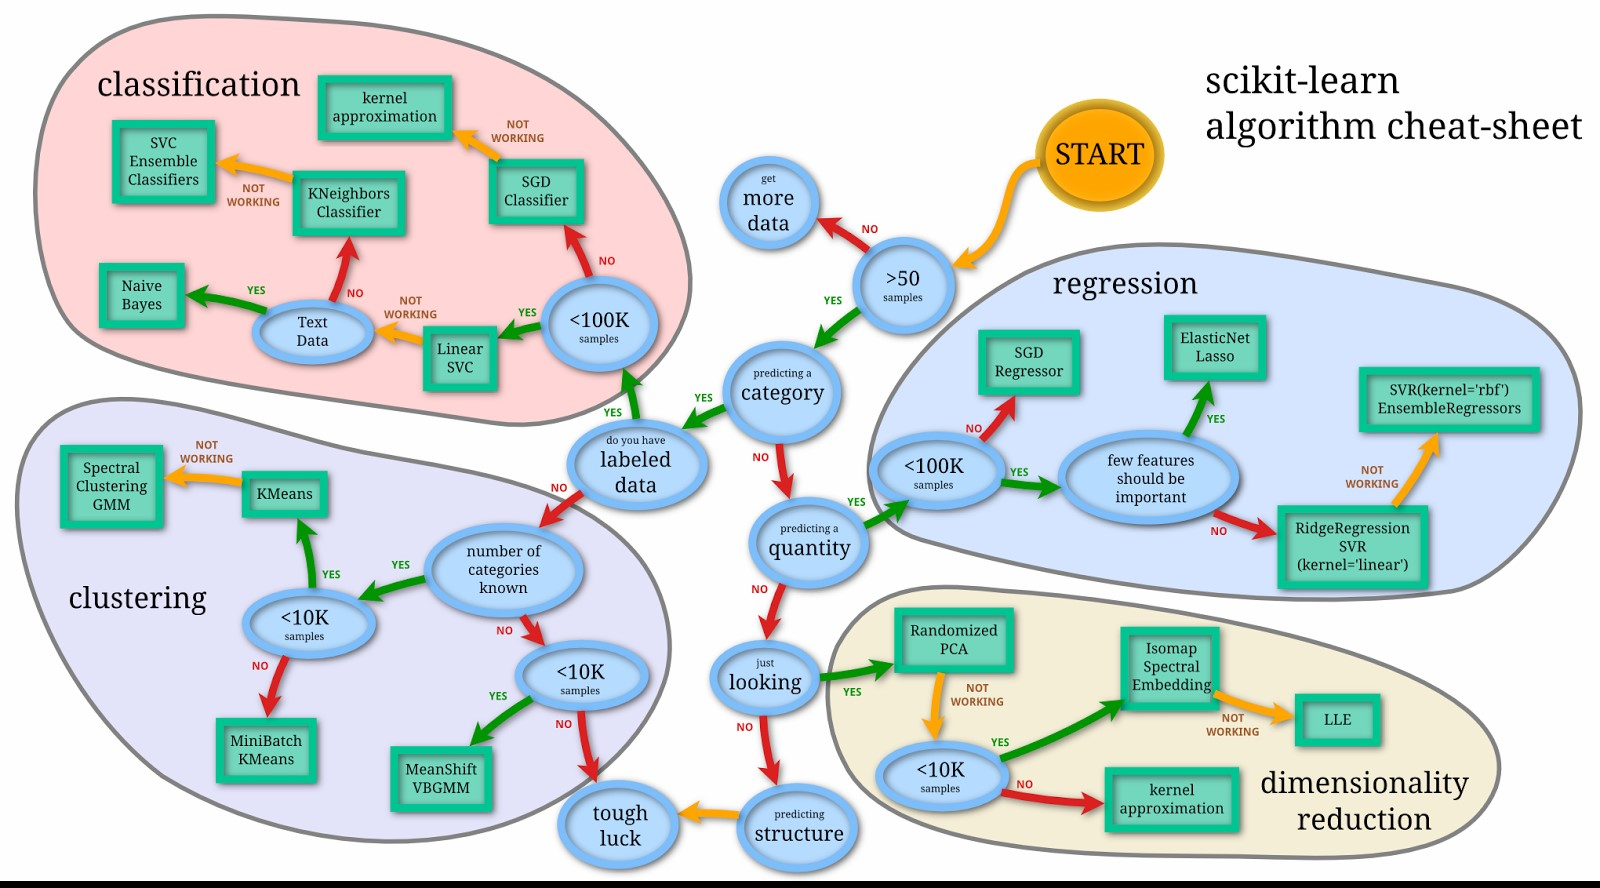
\includegraphics[scale=0.2]{ml1.jpg}
  \caption{scikit-learn algortihm}
  \label{fig:boat1}
\end{figure}
\section{Prerequiste}
Machine Learning is a field of study that gives computers the ability to learn without being explicitly programmed. Machine learning is closely related to (and often overlaps with) computational statistics, which also focuses in prediction-making through the use of computers. Within the field of data analytics, machine learning is method used to devise complex models and algorithms that lend themselves to prediction; in commercial use, this is known as predictive analytics.
\begin{itemize}	
  \item Supervised learning: The computer is presented with example inputs and their desired outputs, given by a "teacher", and the goal is to learn a general rule that maps inputs to outputs
  \item Unsupervised learning: No labels are given to the learning algorithm, leaving it on its own to find structure in its input. Unsupervised learning can be a goal in itself (discovering hidden patterns in data) or a means towards an end (feature learning).
  \item  Reinforcement learning: A computer program interacts with a dynamic environment in which it must perform a certain goal (such as driving a vehicle or playing a game against an opponent). The program is provided feedback in terms of rewards and punishments as it navigates its problem space. 
\end{itemize}

\section{Introduction}

Recommender systems typically produce a list of recommendations in one of two ways through collaborative and content-based filtering or the personality-based approach.Collaborative filtering approaches building a model from a user's past behaviour (items previously purchased or selected and/or numerical ratings given to those items) as well as similar decisions made by other users. This model is then used to predict items (or ratings for items) that the user may have an interest in.Content-based filtering approaches utilize a series of discrete characteristics of an item in order to recommend additional items with similar properties.These approaches are often combined (see Hybrid Recommender Systems).

The differences between collaborative and content-based filtering can be demonstrated by comparing two popular music recommender systems Last.fm and Pandora Radio.

Last.fm creates a "station" of recommended songs by observing what bands and individual tracks the user has listened to on a regular basis and comparing those against the listening behavior of other users. Last.fm will play tracks that do not appear in the user's library, but are often played by other users with similar interests. As this approach leverages the behavior of users, it is an example of a collaborative filtering technique.

Pandora uses the properties of a song or artist (a subset of the 400 attributes provided by the Music Genome Project) in order to seed a "station" that plays music with similar properties. User feedback is used to refine the station's results, deemphasizing certain attributes when a user "dislikes" a particular song and emphasizing other attributes when a user "likes" a song. This is an example of a content-based approach.

Each type of system has its own strengths and weaknesses. In the above example, Last.fm requires a large amount of information on a user in order to make accurate recommendations. This is an example of the cold start problem, and is common in collaborative filtering systems.While Pandora needs very little information to get started, it is far more limited in scope (for example, it can only make recommendations that are similar to the original seed).

Two fundamental challenges for collaborative filtering recommender systems.The first challenge is to improve the scalability of the collaborative filtering algorithms. These algorithms are able to search tens of thousands of potential neighbors in real-time, but the demands of modern systems are to search tens of millions of potential neighbors. Further, existing algorithms have performance problems with individual users for whom the site has large amounts of information.

The second challenge is to improve the quality of the recommendations for the users. Users need recommendations they can trust to help them find items they will like. Users will "vote with their feet" by refusing to use recommender systems that are not consistently accurate for them.In some ways these two challenges are in conflict, since the less time an algorithm spends searching for neighbors, the more scalable it will be, and the worse its quality. For this reason, it is important to treat the two challenges simultaneously so the solutions discovered are both useful and practical.

Recommendations for users are computed by finding items that are similar to other items the user has liked. Because the relationships between items are relatively static,item-based algorithms may be able to provide the same quality as the user-based algorithms with less online computation.

\subsection{Approaches}

\subsubsection{Collaborative filtering}

One approach to the design of recommender systems that has wide use is collaborative filtering.Collaborative filtering methods are based on collecting and analyzing a large amount of information on users behaviors, activities or preferences and predicting what users will like based on their similarity to other users. A key advantage of the collaborative filtering approach is that it does not rely on machine analyzable content and therefore it is capable of accurately recommending complex items such as movies without requiring an "understanding" of the item itself. Many algorithms have been used in measuring user similarity or item similarity in recommender systems. For example, the k-nearest neighbor (k-NN) approach and the Pearson Correlation as first implemented by Allen.

Collaborative filtering is based on the assumption that people who agreed in the past will agree in the future, and that they will like similar kinds of items as they liked in the past.

When building a model from a user's behavior, a distinction is often made between explicit and implicit forms of data collection.

Examples of explicit data collection include the following:

Asking a user to rate an item on a sliding scale,
Asking a user to search,
Asking a user to rank a collection of items from favorite to least favorite,
Presenting two items to a user and asking him/her to choose the better one of them,
Asking a user to create a list of items that he/she likes.

\subsubsection{Content-based filtering}
Another common approach when designing recommender systems is content-based filtering. Content-based filtering methods are based on a description of the item and a profile of the users preference.In a content-based recommender system, keywords are used to describe the items and a user profile is built to indicate the type of item this user likes. In other words, these algorithms try to recommend items that are similar to those that a user liked in the past (or is examining in the present). In particular, various candidate items are compared with items previously rated by the user and the best-matching items are recommended. This approach has its roots in information retrieval and information filtering research.

To abstract the features of the items in the system, an item presentation algorithm is applied. A widely used algorithm is the tf idf representation (also called vector space representation).

To create a user profile, the system mostly focuses on two types of information: 1. A model of the user's preference. 2. A history of the user's interaction with the recommender system.

Basically, these methods use an item profile (i.e., a set of discrete attributes and features) characterizing the item within the system. The system creates a content-based profile of users based on a weighted vector of item features. The weights denote the importance of each feature to the user and can be computed from individually rated content vectors using a variety of techniques. Simple approaches use the average values of the rated item vector while other sophisticated methods use machine learning techniques such as Bayesian Classifiers, cluster analysis, decision trees, and artificial neural networks in order to estimate the probability that the user is going to like the item.

\subsubsection{Hybrid recommender systems}
Recent research has demonstrated that a hybrid approach, combining collaborative filtering and content-based filtering could be more effective in some cases. Hybrid approaches can be implemented in several ways: by making content-based and collaborative-based predictions separately and then combining them; by adding content-based capabilities to a collaborative-based approach (and vice versa); or by unifying the approaches into one model (see for a complete review of recommender systems). Several studies empirically compare the performance of the hybrid with the pure collaborative and content-based methods and demonstrate that the hybrid methods can provide more accurate recommendations than pure approaches. These methods can also be used to overcome some of the common problems in recommender systems such as cold start and the sparsity problem.

Netflix is a good example of the use of hybrid recommender systems. The website makes recommendations by comparing the watching and searching habits of similar users (i.e., collaborative filtering) as well as by offering movies that share characteristics with films that a user has rated highly (content-based filtering).

\section{Objective}
Our project has following objectives.
\begin{itemize}	
  \item Learn research skills such as finding and implementing a research paper.
  \item Understand types of recommender systems
  \item Implement recommender system using K Nearest Neighbour algorithm  
  \item Understand what machine learning is.
  \item Work towards development or applications related to machine learning.
  \item Understand various algorithms used.
  \item Find areas where specific algorithms are useful and where they are not.
\end{itemize}


\section{Pseudo Code of our Algorithm}
Import libraries
Read the dataset
Remove the records when artist is NULL
Calculate the total artist plays
Merge the total artist plays with user data
Choose a threshold for popular artists
Filter only popular artists
Reshape the data for implement the Nearest Neighbour Model 
Fit the model
Make the recommendations

\section{Datasets Used}

The Last.fm data are from the Music Technology Group at the Universitat Pompeu Fabra in Barcelona, Spain. The data were scraped by Òscar Celma using the Last.fm API, and they are available free of charge for non-commercial use.

The Last.fm data are broken into two parts: the activity data and the profile data. The activity data comprises about 360,000 individual users’s Last.fm artist listening information. It details how many times a Last.fm user played songs by various artists. The profile data contains each user’s country of residence.

\section{Libraries Used}
1. Numpy

NumPy is the fundamental package for scientific computing with Python. It contains among other things:

  -  a powerful N-dimensional array object
  -  sophisticated (broadcasting) functions
  -  tools for integrating C/C++ and Fortran code
  -  useful linear algebra, Fourier transform, and random number capabilities

Besides its obvious scientific uses, NumPy can also be used as an efficient multi-dimensional container of generic data. Arbitrary data-types can be defined. This allows NumPy to seamlessly and speedily integrate with a wide variety of databases.

NumPy is licensed under the BSD license, enabling reuse with few restrictions.

2. Pandas

Python Data Analysis Library

pandas is an open source, BSD-licensed library providing high-performance, easy-to-use data structures and data analysis tools for the Python programming language.


3. scikit-learn
Machine Learning library in Python

  -  Simple and efficient tools for data mining and data analysis
  -  Accessible to everybody, and reusable in various contexts
  -  Built on NumPy, SciPy, and matplotlib
  -  Open source, commercially usable - BSD license


\section{PROCESS MODEL}
\begin{figure}[H]

\begin{center}

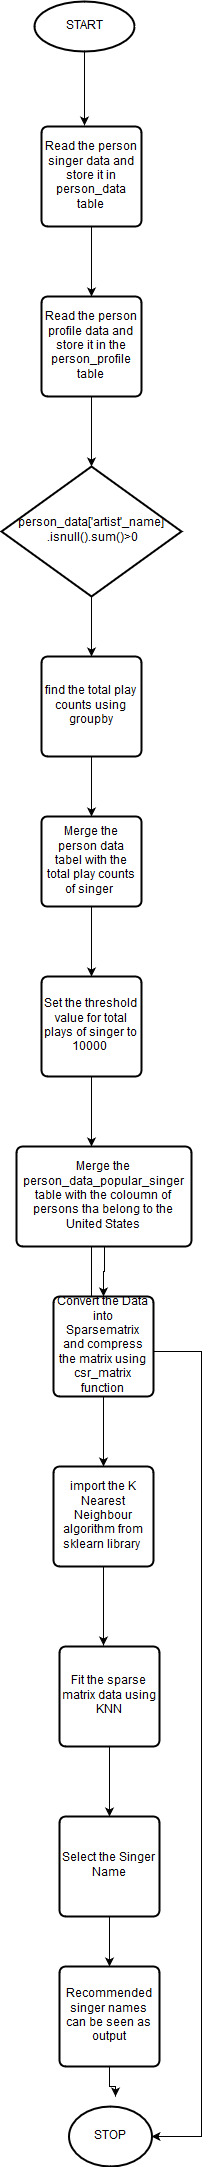
\includegraphics[scale=.3]{process_model.jpg}

 \end{center}

  \caption{Process Model}

  \label{fig:}

\end{figure}

\section{K-Nearest Neighbours}

In pattern recognition, the k-nearest neighbors algorithm (k-NN) is a non-parametric method used for classification and regression.[1] In both cases, the input consists of the k closest training examples in the feature space. The output depends on whether k-NN is used for classification or regression:

In k-NN classification, the output is a class membership. An object is classified by a majority vote of its neighbors, with the object being assigned to the class most common among its k nearest neighbors (k is a positive integer, typically small). If k = 1, then the object is simply assigned to the class of that single nearest neighbor.

In k-NN regression, the output is the property value for the object. This value is the average of the values of its k nearest neighbors.

%%% End document
\end{document}